% Options for packages loaded elsewhere
\PassOptionsToPackage{unicode}{hyperref}
\PassOptionsToPackage{hyphens}{url}
\PassOptionsToPackage{dvipsnames,svgnames*,x11names*}{xcolor}
%
\documentclass[
]{article}
\usepackage{lmodern}
\usepackage{amssymb,amsmath}
\usepackage{ifxetex,ifluatex}
\ifnum 0\ifxetex 1\fi\ifluatex 1\fi=0 % if pdftex
  \usepackage[T1]{fontenc}
  \usepackage[utf8]{inputenc}
  \usepackage{textcomp} % provide euro and other symbols
\else % if luatex or xetex
  \usepackage{unicode-math}
  \defaultfontfeatures{Scale=MatchLowercase}
  \defaultfontfeatures[\rmfamily]{Ligatures=TeX,Scale=1}
\fi
% Use upquote if available, for straight quotes in verbatim environments
\IfFileExists{upquote.sty}{\usepackage{upquote}}{}
\IfFileExists{microtype.sty}{% use microtype if available
  \usepackage[]{microtype}
  \UseMicrotypeSet[protrusion]{basicmath} % disable protrusion for tt fonts
}{}
\makeatletter
\@ifundefined{KOMAClassName}{% if non-KOMA class
  \IfFileExists{parskip.sty}{%
    \usepackage{parskip}
  }{% else
    \setlength{\parindent}{0pt}
    \setlength{\parskip}{6pt plus 2pt minus 1pt}}
}{% if KOMA class
  \KOMAoptions{parskip=half}}
\makeatother
\usepackage{xcolor}
\IfFileExists{xurl.sty}{\usepackage{xurl}}{} % add URL line breaks if available
\IfFileExists{bookmark.sty}{\usepackage{bookmark}}{\usepackage{hyperref}}
\hypersetup{
  colorlinks=true,
  linkcolor=blue,
  filecolor=Maroon,
  citecolor=Blue,
  urlcolor=Blue,
  pdfcreator={LaTeX via pandoc}}
\urlstyle{same} % disable monospaced font for URLs
\usepackage{longtable,booktabs}
% Correct order of tables after \paragraph or \subparagraph
\usepackage{etoolbox}
\makeatletter
\patchcmd\longtable{\par}{\if@noskipsec\mbox{}\fi\par}{}{}
\makeatother
% Allow footnotes in longtable head/foot
\IfFileExists{footnotehyper.sty}{\usepackage{footnotehyper}}{\usepackage{footnote}}
\makesavenoteenv{longtable}
\setlength{\emergencystretch}{3em} % prevent overfull lines
\providecommand{\tightlist}{%
  \setlength{\itemsep}{0pt}\setlength{\parskip}{0pt}}
\setcounter{secnumdepth}{-\maxdimen} % remove section numbering
\ifluatex
  \usepackage{selnolig}  % disable illegal ligatures
\fi

\author{}
\date{}

\begin{document}

\newcommand{\Ber}{\operatorname{Ber}}
\newcommand{\E}{\operatorname{E}}
\newcommand{\V}{\operatorname{Var}}
\newcommand{\diag}{\operatorname{diag}}

\newcommand{\bi}{\mathbf{i}}
\newcommand{\bj}{\mathbf{j}}
\newcommand{\bt}{\mathbf{t}}

\newcommand{\bw}{{\boldsymbol{w}}}
\newcommand{\bv}{{\boldsymbol{v}}}
\newcommand{\bx}{{\boldsymbol{x}}}
\newcommand{\by}{{\boldsymbol{y}}}
\newcommand{\bb}{{\boldsymbol{b}}}
\newcommand{\bz}{{\boldsymbol{z}}}
\newcommand{\bu}{{\boldsymbol{u}}}
\newcommand{\bX}{{\boldsymbol{X}}}
\newcommand{\bY}{{\boldsymbol{Y}}}
\newcommand{\bZ}{{\boldsymbol{Z}}}

\hypertarget{logistic-regression}{%
\section{Logistic Regression}\label{logistic-regression}}

\hypertarget{maximum-likelihood}{%
\subsection{Maximum Likelihood}\label{maximum-likelihood}}

Suppose that there is a coin which you think is biased. You flip the
coin 10 times and get 7 heads. Based on this \emph{training data} set,
what is the probability that the next flip will show heads? Can you
justify your answer? To provide a rigorous argument for the answer, we
can use \emph{maximum likelihood} estimation.

Let \(y\) be the (unknown) probability that the biased coin shows heads.
Since there are only two possible results, heads or tails, the
experiment of flipping the coin is a \emph{Bernoulli trial}. We
introduce a \emph{Bernoulli random variable} \(T\) such that
\[ T=\begin{cases} 1 & \text{ if the coin shows heads}, \\ 0 & \text{ otherwise}. \end{cases} \]
with probabilities
\[ P(T=1|y)=y \quad \text{ and } \quad P(T=0|y)=1-y, \quad \text{respectively}. \]\\
The probability mass function \(\operatorname{Ber}(t|y)\) of \(T\) can
be written in a compact way
\[ \operatorname{Ber}(t|y)= y^t (1-y)^{1-t}, \quad t=0,1. \]

Suppose that we have a data set \(\mathcal D = \{ t_1, \dots, t_N \}\)
of observed values of \(t \in \{ 0,1 \}\) from \(N\) coin flips. Let
\(p(\mathcal D|y)\) denote the probability of getting the set
\(\mathcal D\), given that \(y\) is the probability of the biased coin.
Since each flip is independent, the probability \(p(\mathcal D|y)\) is
equal to the product of the probabilities of individual flip results,
i.e.~it is equal to
\[ p(\mathcal D| y) = \prod_{n=1}^N \operatorname{Ber}(t_n|y) = \prod_{n=1}^N y^{t_n} (1-y)^{1-t_n}. \]

This is a function of \(y\); as \(y\) varies, the function
\(p(\mathcal D|y)\) produces probabilities of the set \(\mathcal D\)
determined by \(y\). When \(p(\mathcal D|y)\) is maximized at a value
\(y_{\mathrm {ML}}\), we can say that \(y_{\mathrm{ML}}\) has maximum
likelihood based on the data st \(\mathcal D\). This leads to

\[\text{ Task: Estimate a value $y_{\mathrm{ML}}$ that maximizes $p(\mathcal D|y)$}.\]

This is a Calculus problem. We will have to take the derivative of the
function. Before taking the derivative, we notice that the expression of
\(p(\mathcal D|y)\) is a product of exponentials. In such a situation,
logarithmic differentiation can be used to ease the process of
differentiation, and the function can be replace by
\[ \ln p(\mathcal D|y) = \sum_{n=1}^N \{ t_n \ln y + (1-t_n) \ln(1-y)\} .\]

Now we take the derivative of the function with respect to \(y\), set
the derivative equal to \(0\) to obtain a critical value, and check if
the critical value \(y_{\mathrm{ML}}\) indeed maximizes the function.
The result is \[ y_{\mathrm{ML}}= \frac 1 N \sum_{n=1}^N t_n ,\] which
is the \emph{sample mean}. This justifies our guess for a biased coin in
a rigorous way.

\textbf{Exercises}: Provide details to obtain \(y_{\mathrm{ML}}\).

\hypertarget{logistic-regression-1}{%
\subsection{Logistic Regression}\label{logistic-regression-1}}

Suppose that there is a certain test (similar to GRE) for undergraduate
students who apply for a graduate program. The test score is used for
admission decisions as one of the credentials that students provide. The
table below shows the test scores of 10 students and the results of
admission decisions:

\begin{longtable}[]{@{}llcccccccccc@{}}
\toprule
\(x\) & : & \(272\) & \(331\) & \(295\) & \(287\) & \(315\) & \(266\) &
\(303\) & \(294\) & \(317\) & \(309\)\tabularnewline
\midrule
\endhead
\(t\) & : & 0 & 1 & 1 & 0 & 1 & 0 & 0 & 0 & 1 & 1\tabularnewline
\bottomrule
\end{longtable}

\(x\) test score \(t=1\) accepted \(t=0\) rejected

There is a student whose test score is 299. Based on this data, what is
the probability that the student will be accepted? If the probability is
greater than 0.5, we can \emph{classify} the student as \emph{Likely
Accepted}; if the probability is less than 0.5, as \emph{Likely
Rejected}. This type of problem is called \emph{classification} problem
in machine learning.

An answer to this problem would have a procedure to produce probability
\(y\) from a test score \(x\). A typical way to obtain a number between
0 and 1 (that is to be considered as probability) from an arbitrary real
number is to use a function whose graph is an \(S\)-shaped curve, called
a \emph{sigmoid} function. One of the most common sigmoid functions is
the \emph{logistic} function
\[ \sigma(x) = \frac {e^x}{e^x+1}= \frac 1 {1+e^{-x}}.\]

\begin{center}
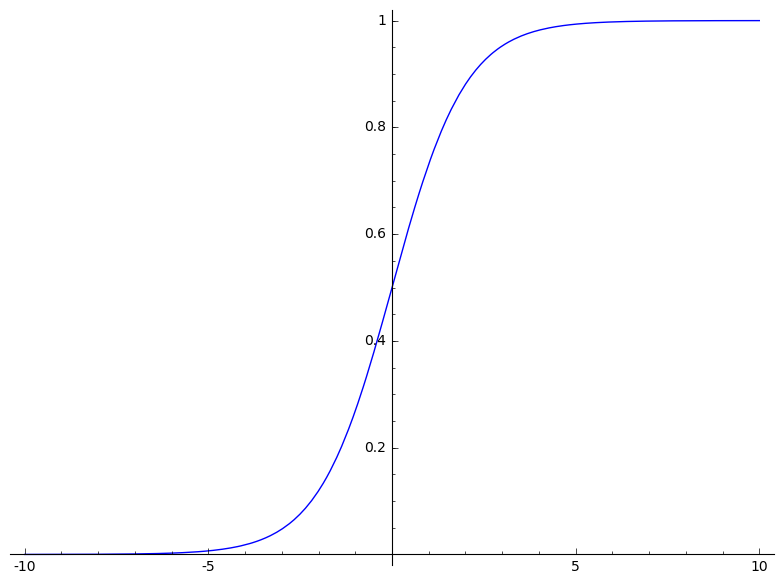
\includegraphics[scale=0.2]{sigmoid}

Graph of the Logistic Function


\end{center}

Clearly, the logistic function converts \((-\infty, \infty)\) to
\((0,1)\). In particular, the value \(0\) corresponds to \(0.5\). In
order to apply this function to\\
a data set \(\{ x_1, x_2, \dots , x_N \}\) of test scores, we need to
first adjust the values \(x_n\) in accordance with the logistic function
in such a way that the result will best fit for the given data. Here we
make an assumption that the adjustment is done by a linear function of
the form \(w_1 x_n+w_2\) so that the probability is given by
\begin{equation} \label{eqn-y-sigma} y_n=\sigma(w_1 x_n +w_2). \end{equation}
This is the same kind of assumption we made for linear regression.

Now the question is how to find the best values of \(w_0\) and \(w_1\).
Let us consider the likelihood of the given data set. Each score \(x\)
corresponds to probability \(y\) and a student with score \(x\) will be
accepted with probability \(y\) through a Bernoulli trial. It is like
flipping a biased coin with probability \(y\). Given a data set
\(\mathcal D=\{(x_n, t_n) \}\), \(t_n \in \{ 0,1 \}\),
\(n=1, \dots, N\), we compute the likelihood of this data set and obtain
\[ p(\mathcal D|{\boldsymbol{w}}) =  \prod_{n=1}^N \operatorname{Ber}(t_n|y_n) = \prod_{n=1}^N y_n^{t_n} (1-y_n)^{1-t_n}, \]
where \(y_n= \sigma(w_1 x_n+w_2)\) and \({\boldsymbol{w}}=(w_1, w_2)\).
The best choice of \({\boldsymbol{w}}=(w_1,w_2)\) would make this
likelihood the largest possible. Thus our task can be summarized as the
following.

\[\text{Task: Determine ${\boldsymbol{w}}$ that maximize the likelihood $p(\mathcal D|{\boldsymbol{w}})$.}\]

Test scores make only one feature in credentials for admission
decisions. Assume that there are \(k\) different features.\\
Then the \(n^\mathrm{th}\) student provides credentials
\(\{x_{n1}, x_{n2}, \dots , x_{nk} \}\), and as in linear regression,
the credentials of \(N\) student can be arranged into a matrix
\[  \begin{bmatrix} x_{11} & x_{12} & \cdots & x_{1k} \\ x_{21} & x_{22} & \cdots & x_{2k} \\ \vdots & \vdots & & \vdots \\ x_{N1} & x_{N2} & \cdots & x_{Nk} \end{bmatrix} .\]

The function in \eqref{eqn-y-sigma} is now generalized to
\[ y_n=\sigma(w_1 x_{n1}+ w_2 x_{n2} + \cdots + w_k x_{nk}+w_{k+1} ), \]
which can be rewritten in vector notations
\[ y_n= \sigma( {\boldsymbol{x}}_n{\boldsymbol{w}}) ,\] where
\({\boldsymbol{w}}=(w_1, w_2, \dots , w_k, w_{k+1})^\top\) is a column
vector to be determined and
\({\boldsymbol{x}}_n=(x_{n1}, x_{n2}, \dots, x_{nk}, 1)\). With
\(y_n=\sigma({\boldsymbol{x}}_n {\boldsymbol{w}})\), the expression of
the likelihood \(p(\mathcal D| {\boldsymbol{w}})\) does not change.

To make differentiation easier, we take the logarithm of the likelihood
and want to determine \({\boldsymbol{w}}\) which maximizes
\[ \ln p(\mathcal D|{\boldsymbol{w}}) = \sum_{n=1}^N \{ t_n \ln y_n + (1-t_n) \ln (1-y_n)\} ,\]
or equivalently, \({\boldsymbol{w}}\) which minimizes
\[ E({\boldsymbol{w}}):=-\ln p(\mathcal D|{\boldsymbol{w}}) = -\sum_{n=1}^N \{ t_n \ln y_n + (1-t_n) \ln (1-y_n)\} .\]
This problem is called \emph{logistic regression}.

Unlike linear regression, it is difficult to find closed form formulas
for solutions to this problem. Instead, we will use an inductive process
to approximate the vector \({\boldsymbol{w}}\). We will study two
standard methods for this purpose, called \emph{Gradient Descent} and
\emph{Newton's Method}.

\hypertarget{applying-newtons-method-to-the-logistic-regression}{%
\subsection{Applying Newton's method to the logistic
regression:}\label{applying-newtons-method-to-the-logistic-regression}}

\[ E ({\boldsymbol{w}}) = - \ln p(t|{\boldsymbol{w}}) = - \sum_{n=1}^N \{ t_n \ln y_n + (1-t_n) \ln (1-y_n)\},  \]
where
\(y_n=\sigma(a_n)=\sigma({\boldsymbol{x}}_n^\top {\boldsymbol{w}})\).
Note that \(\sigma'(x) =\sigma(x)(1-\sigma(x))\).

\begin{itemize}
\item
  We obtain
  \[ \nabla E({\boldsymbol{w}})= \sum_{n=1}^N (y_n-t_n){\boldsymbol{x}}_n = X ({\boldsymbol{y}}-\mathbf{t}), \]
  where
  \[ X=\begin{bmatrix} 1 &1 & \cdots &1 \\ x_1 & x_2 & \cdots &x_N \\ x_1^2 & x_2^2 & \cdots &x_N^2 \\ \vdots & \vdots & & \vdots \\ x_1^D & x_2^D & \cdots &x_N^D \\\end{bmatrix}, \quad {\boldsymbol{y}}=\begin{bmatrix} y_1 \\ y_2 \\ \vdots \\ y_N \end{bmatrix}, \quad \text{ and } \mathbf{t}= \begin{bmatrix} t_1 \\ t_2 \\ \vdots \\ t_N \end{bmatrix} . \]
\item
  We also get
  \[ \mathbf H = \sum_{n=1}^N y_n(1-y_n) {\boldsymbol{x}}_n {\boldsymbol{x}}_n^\top = X R X^\top, \]
  where \(R=\operatorname{diag}( y_n(1-y_n))\).
\item
  Then we have
  \[ \boxed{{\boldsymbol{w}}_{k+1} = {\boldsymbol{w}}_k - (X R X^\top)^{-1} X ({\boldsymbol{y}}-\mathbf{t}) },\]
  where \(R\) and \({\boldsymbol{y}}\) are determined by
  \({\boldsymbol{w}}_k\) in each step.
\end{itemize}

\hypertarget{example-test-scores-and-admission-to-a-graduate-school}{%
\subsubsection{Example: Test scores and admission to a graduate
school}\label{example-test-scores-and-admission-to-a-graduate-school}}

\begin{itemize}
\item
  Chose \(D=1\). Then \(a_n=w_0+w_1x_n\). \textbackslash{} From the
  data, we have \[X= \begin{bmatrix}  1 &1 &1 &1 &1 &1 &1 &1 &1 &1 \\
  272&331&295&287&315&266&303&294&317&309 \end{bmatrix}, \] and
  \[ \mathbf{t}=[0,1,1,0,1,0,0,0,1,1]^\top .\]
\item
  Choose \({\boldsymbol{w}}_0=(0,0)^\top\). Then \({\boldsymbol{w}}_k\)
  converges to \[ (-57.2937, 0.1910)^\top .\]
\item
  If \(x=299\), then the probability of admission is
  \[ y= \sigma(-57.2937+ 0.1910*299) \approx 0.454 .\]
\end{itemize}

\end{document}
